\documentclass[12pt, a4paper]{report}
\usepackage[utf8]{inputenc}
\usepackage[swedish]{babel}
\usepackage{fullpage}
\usepackage{hyperref}
\usepackage{amsmath}
\usepackage{graphicx}
\title{Beräkningsvetenskap och analys 1TD333\\Miniprojekt 1}
\author{Erik Englund, Martin Johansson, Oskar Persson}

\begin{document}
\maketitle
\chapter{Del 1}
\section{Härledning av ekvationssystem}

$$P_1 = 10$$
$$P_5 = 0$$
$$P_6 = 0$$
$$Q_j = k \cdot L(P_{in} - P_{ut})$$
$$Q_1 = Q_2 + Q_3\;\;(1)$$
$$Q_3 = Q_4 + Q_6\;\;(2)$$
$$Q_5 = Q_2 + Q_4\;\;(3)$$
\newline
$(1):\;\;\; 0.001\cdot300(P_1-P_2)=(0.001\cdot500(P_2-P_4))+(0.001\cdot500(P_2-P_3))$
$$\Rightarrow0.3P_1-0.3P_2=0.5P_2-0.5P_4+0.5P_2-0.5P_3$$
\newline
$(2):\;\;\; 0.001\cdot500(P_2-P_3)=(0.001\cdot600(P_3-P_4))+(0.001\cdot500(P_3-P_6))$
$$\Rightarrow0.5P_2-0.5P_3=0.6P_3-0.6P_4+0.5P_3-0.5P_6$$
$$\Rightarrow0.5P_2-0.5P_3=1.1P_3-0.6P_4-0.5P_6$$
$$\Rightarrow0.5P_2-1.6P_3+0.6P_4+0.5P_6=0$$
\newline
$(3):\;\;\; 0.001\cdot500(P_2-P_4)+0.001\cdot600(P_3-P_4)=(0.001\cdot500(P_4-P_5))$
$$\Rightarrow0.5P_2-0.5P_4+0.6P_3-0.6P_4=0.5P_4-0.5P_5$$
$$\Rightarrow0.5P_2+0.6P_3-1.1P_4=0.5P_4-0.5P_5$$
$$\Rightarrow0.5P_2+0.6P_3-1.6P_4+0.5P_5=0$$

\section{graf från del 1}

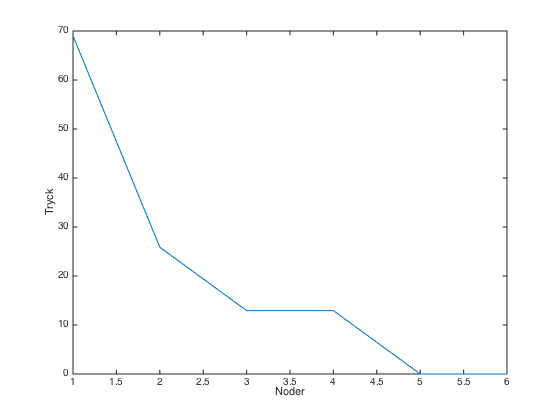
\includegraphics{del1_plot.png}

\section{Medeltrycksberäkning}

Se bifogad kod.

\section{Hur gör man beräkningarna effektiva?}

Med hjälp av \textbf{LU-faktorisering}.

\chapter{Del 2}

Se bifogad kod.

\end{document}
